\chapter{Introdução}\label{cap:introducao}

\section{Considerações Iniciais}
Após um terremoto, para aumentar as chances de sobrevivência das vitimas,
é fundamental prestar assistência médica nas primeiras 24 horas \cite{schultz1996medical}.
A dificuldade de realizar busca em meio a escombros, a baixa acessibilidade terrestre devido a danos na malha rodoviárias e o número limitado de equipes de busca são fatores que influenciam no andamento de uma missão de salvamento.
Para auxiliar as missões de resgate, robôs estão sendo cada vez mais empregados. Entretanto, um dos obstáculos a serem superados está em como levar esses dispositivos até sua área de atuação. 

Uma maneira promissora é o transporte aéreo até as regiões de interesse seguido do envio por paraquedas até o solo. 
O salto de paraquedas pode ser divido em três fases: o salto do avião, a abertura do paraquedas e a aterrissagem ao solo.
Este último se mostra o mais complexo devido às acelerações de impacto, que podem danificar os componentes frágeis de um robô durante um aterrissagem \cite{tsujita2017drop}.
Breves estudos mostraram a redução de impacto ao solo quando se utilizam materiais acolchoados \cite{tsujita2017drop} \cite{tsujita2017analysis}.
Este trabalho tem como objetivo dar continuidade a esses trabalhos, medindo a eficiência de tipos distintos de materiais acolchoados, na construção de um simulador de testes de queda, além da identificação de parâmetros de amortecimento de \textit{Rayleigh}.

Desastres naturais são eventos geológicos ou atmosféricos que possuem grande impacto econômico e social. Pode-se citar como exemplo: furacões, terremotos, tufões, tsunamis, deslizamentos, erupções vulcânicas e inundações\cite{naturaldisasters}.
Além do alto número de mortes e feridos, existem os danos às construções como escolas, fábricas, hospitais, na infraestrutura e produção rural\cite{benson1997economic}.
Dentre os maiores desastres naturais que ocorreram na última década, tem-se em 2010, o terremoto de magnitude 7.0 que atingiu o Haiti, causando cerca de 230.000 mortes, 300.000 feridos e um prejuízo avaliado em cerca de 8 bilhões de dólares\cite{haiti2010}.
No ano seguinte, em 2011, a região leste do Japão sofreu com um terremoto de magnitude 9.1 e o consequente tsunami. O incidente levou o falecimento de cerca de 16.000 pessoas, com um prejuízo avaliado em 199 bilhões de dólares \cite{tohoku2011}.
O mesmo país sofreu, em 2019, com o tufão de categoria 5, \textit{Hagibis}, que causou deslisamentos e inundações, levando a um prejuízo estimado em 10 bilhões de dólares, além 85 mortes e dezenas de desabrigados \cite{hagibis2019}.

Eventos como terremotos são dificilmente previstos \cite{kagan1997earthquakes}, além de não poderem ser evitados nem controlados\cite{office1995reducing}.
Desse modo, a prevenção é a maneira mais efetiva para reduzir os prejuízos causados por desastres naturais \cite{durkin1992improving}. Umas das estratégias preventivas é a construção de estruturas com tecnologias que permitam atuar em condições mais extremas. No Japão, prédios com pêndulos\cite{nagase2000earthquake} e amortecedores \cite{takewaki2011smart} estão sendo construídos preparados para absorver as vibrações de terremotos; para conter o avanço das ondas, barragens são construídas em litorais.\cite{kamphuis2010introduction}; pavimentos permeáveis podem ser instalados em áreas urbanas com o objetivo de reduzir a ocorrência de inundações.\cite{selbig2018evaluating}

Tais medidas apenas mitigam os prejuízos mas não o extinguem.
Após a passagem de um terremoto, escombros e destroços podem aprisionar e causar ferimentos às vitimas. Nesse cenário, ter uma resposta médica rápida e eficiente é fundamental para garantir a sobrevivência desses pacientes. Estudos mostraram que 25\% a 50\% das vítimas de soterramento poderiam ser salvas se assistência médica fossem prestada a tempo. Durante terremotos, 85\% a 95\% das vítimas que sobreviveram foram socorridas nas primeiras 24 horas após o terremoto \cite{schultz1996medical}.
O atendimento às vítimas pode ser comprometido pelos danos causados na malha rodoviária de uma região, na qual ruas são obstruídas e destroços de prédios dificultam a acessibilidade nessas áreas. Além disso, a quantidade de recurso disponibilizado para a busca, a dificuldade em localizar vítimas em meio a escombros e o risco de enviar equipes de busca em edifícios em risco de desabamento resultam em tempo de resgate longos. 

Uma das formas de diminuir esse tempo esta no uso de robôs para auxiliarem no resgate das vítimas. O uso destas tecnologias nesse cenário teve início com os ataques do 11 de setembro, no \textit{World Trade Center}, onde pequenos dispositivos, chamados de \textit{packbots}, mostrado na figura \ref{fig:packbot}, foram utilizados na busca de vítimas que pudessem estar presas em escombros de prédios. Esses robôs atuaram em locais instáveis, que poderiam comprometer a vida das equipes médicas caso fizessem a busca pessoalmente\cite{murphy2004trial}. Essa tragédia marcou o surgimento do uso de robôs para busca e resgate e, deste então, estão cada vez mais presentes, principalmente em missões de difícil acesso ou nocivos para humanos.


 \begin{figure}[H]
        \centering
        \caption{Robô \textit{packbot} que auxiliou o resgate das vitimas do 11 de setembro.}
        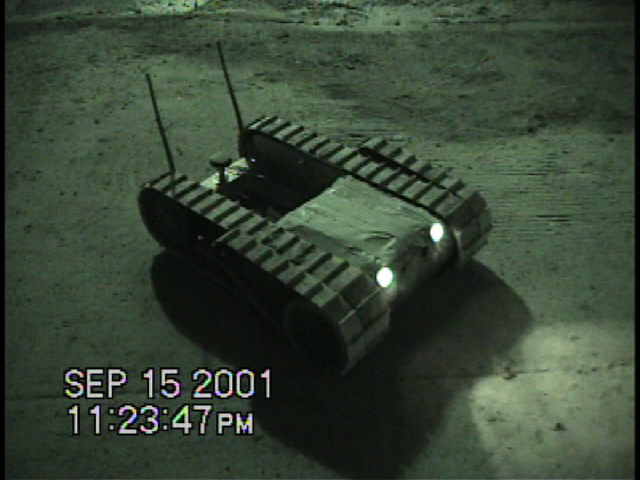
\includegraphics[width=8cm]{./figs/packbot.jpg}
        \par\medskip
Fonte: https://nsf.gov/news/mmg/media/images/packbot6\_f\_7e432d6d-ab16-4b4f-8944-0d89a8bef999.jpg
        \label{fig:packbot}
\end{figure}

O terremoto e tsunami que atingiram o Japão em 2011 teve grande impacto na Central Nuclear de \textit{Fukushima Daiichi}. A perda de energia devido ao desastre natural gerou explosões de hidrogênio na usina nuclear, na qual três reatores foram danificados. Em um deles, os danos foram tão profundos, que houve vazamento de material radioativo, com possível contaminação do Oceano Pacífico. Devido ao alto nível de radiação, não seria possível intervenção humana sem que houvesse riscos de vida.
Desse modo, para poder analisar os danos existentes dentro da usina nuclear e conter o vazamento de água contaminada o uso de um dispositivo remotamente controlado era indispensável.
Em um cenário de urgência, a \textit{New Energy and Industrial Technology Development Organization} (NEDO) e a \textit{}{Tokyo Electric Power Company (TEPCO)} juntaram esforço no projeto do robô Quince, mostrado na figura \ref{fig:quince}, que atuou nas missões na Usina Nuclear de \textit{Fukushima Daiichi} \cite{nagatani2013emergency}.

 \begin{figure}[H]  
        \centering
        \caption{Robô \textit{}{Quince} que atuau nas 6 missões de Usina Nuclear de \textit{Fukushima Daiichi}.}
        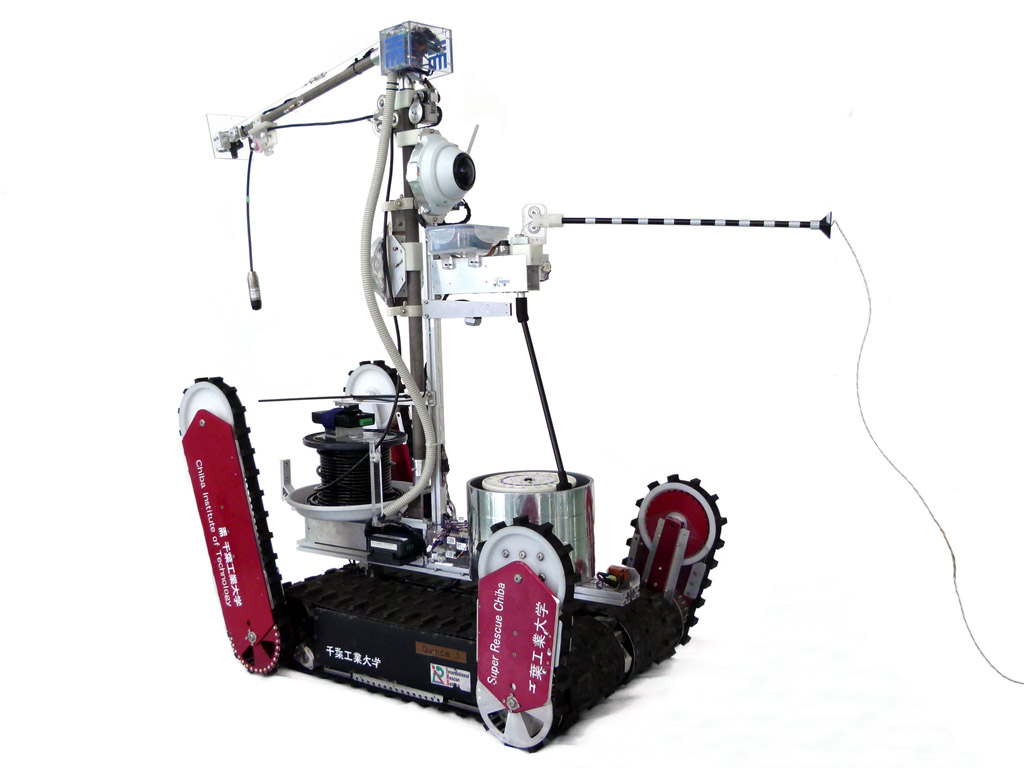
\includegraphics[width=8cm]{./figs/quince.jpg}
        \label{fig:quince}
\end{figure}

Em 2019, durante o incêndio na catedral de \textit{Notre Dame}, um robô remotamente controlado chamado de \textit{Colossus}, mostrado na figura \ref{fig:colossus2019}, foi utilizado para extinguir chamas de áreas que poderiam comprometer a vida de bombeiros\cite{colossus2019}.

 \begin{figure}[h]  
        \centering
        \caption{Robô \textit{}{Colossus} utilizado no controle de chamas.}
        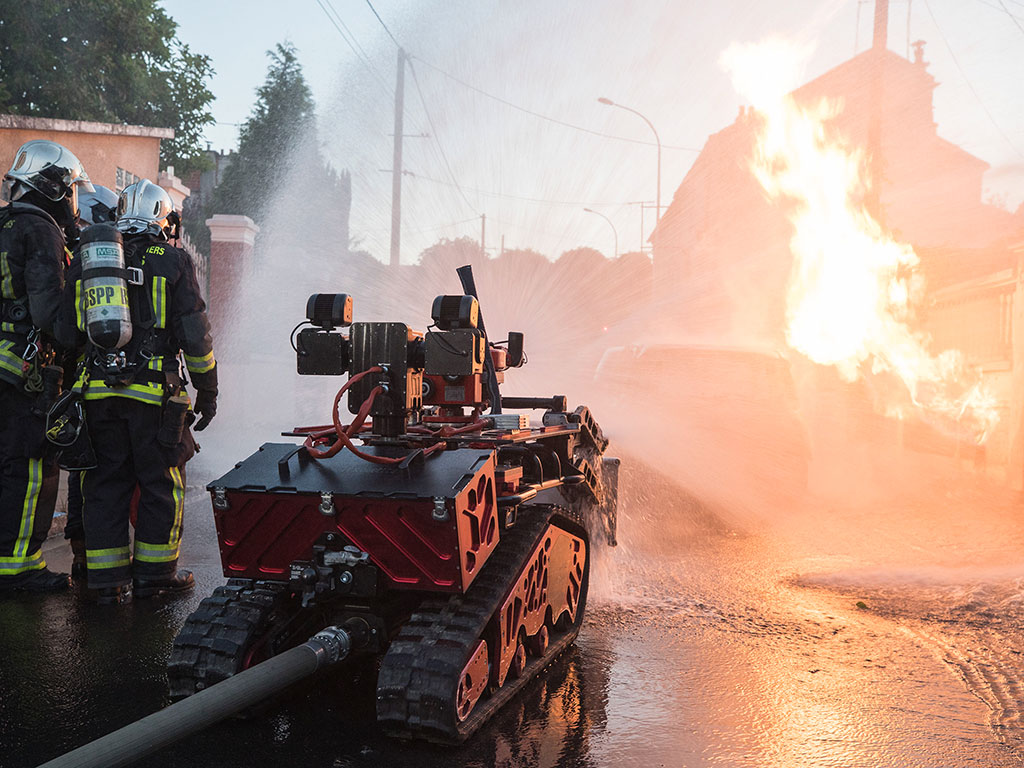
\includegraphics[width=8cm]{./figs/colossus2019.jpg}
        \par\medskip
Fonte: https://robots.ieee.org/robots/quince/
        \label{fig:colossus2019}
\end{figure}
%https://robots.ieee.org/robots/colossus/

%https://builtin.com/robotics/rescue-robots

No mesmo ano, a \textit{Boston Dynamics} apresentou a nova versão de seu robô humanoide, \textit{Atlas}, mostrado na figura \ref{fig:atlas}. Diferentemente dos outros robôs, destacados previamente, o \textit{Atlas} possui alta mobilidade, podendo se locomover eficientemente em diferentes terrenos além de segurar objetos \cite{atlas}.

 \begin{figure}[H]  
        \centering
        \caption{Robô \textit{Atlas} da \textit{Boston Dynamics}.}
        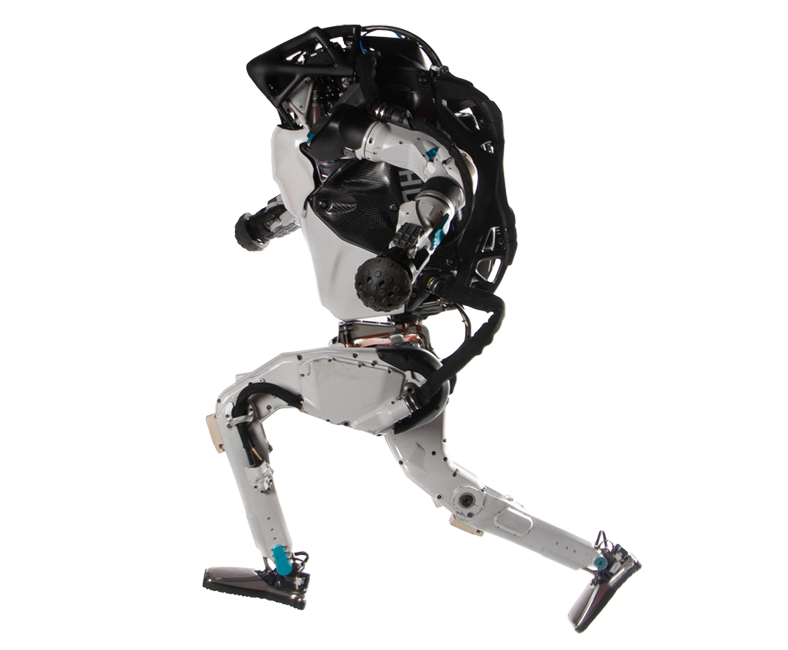
\includegraphics[width=8cm]{./figs/atlas.png}
        \par\medskip
Fonte: https://www.bostondynamics.com/atlas
        \label{fig:atlas}
\end{figure}

Uma das dificuldades do uso de robôs em missões de resgate esta no transporte desses dispositivos para suas área de atuação. No caso de terremotos, a obstrução de vias pode dificultar o acesso terrestre, que já é um obstáculo para as equipes médicas. Umas possível solução esta no transporte aéreo, na qual robôs podem ser enviados em aviões ou helicópteros e entregados por meio de paraquedas.
Esta solução possui alguns obstáculos a serem superados, um deles se encontra durante a fase de aterrissagem. Mesmo com a desaceleração proveniente do paraquedas, o impacto ao solo ainda é alto. Com uma força de aterrissagem média de 11$kN$, o risco de lesão é de 6 a cada 1000 aterrissagens, podendo aumentar quando a aterrissagem é feita incorretamente \cite{whitting2007parachute}.
Para robôs, essas lesões se traduzem como danos ao equipamentos e componentes frágeis, como visto em \cite{tsujita2017drop}.
Estudos realizados com robôs de uma perna, mostraram uma redução na aceleração de impacto quando uma postura semi-sentada é adotada\cite{tsujita2017drop}. Adicionalmente,
breves estudos mostraram a performance do uso de materiais acolchoados na redução das acelerações de impacto ao solo \cite{tsujita2017drop} \cite{tsujita2017analysis}.
Desse modo, mostra-se interessante a continuidade deste trabalho, com uma análise mais profundada no uso de materiais acolchoados em testes de queda. Adicionalmente, a construção de um simulador de testes de queda se mostra essencial, uma vez que os experimentos nas pesquisas mencionadas são realizados a um alto custo financeiro. Realizar repetidos testes de queda em robôs humanoides é inviável dado a perspectiva de danificá-los devido ao impacto ao solo, como mostrado em \cite{tsujita2017drop}.

%https://singularityhub.com/2019/04/12/ai-and-robotics-are-transforming-disaster-relief/

%https://builtin.com/robotics/rescue-robots

%https://onlinelibrary.wiley.com/doi/full/10.1046/j.1442-2026.2001.00201.x

%https://journals.lww.com/co-criticalcare/fulltext/2005/12000/Disaster_management_teams.13.aspx

%https://www.student.cs.uwaterloo.ca/~cs492/papers/trial.pdf

\section{Objetivos}

Este trabalho tem como objetivo a análise do envio de robôs humanoides em áreas de baixa acessibilidade terrestre utilizando aterrissagem por paraquedas e materiais acolchoados para reduzir as acelerações de impacto.
Como objetivos específicos, têm-se modelar um simulador dinâmico para o experimentos de testes de queda, analisar o desempenho dos amortecimentos em reduzir as acelerações de impacto e identificar os parâmetros de Rayleigh para os materiais utilizados nos testes de queda.

\section{Materiais e Métodos}

O trabalho se inicia com uma contextualização, justificando o problema a ser estudado, apresentando estudos e pesquisas relevantes sobre o tema.
A seguir, serão apresentados aspectos gerais \textit{Métodos dos Elementos Finitos} (MEF) e \textit{Dinâmica de Multicorpos} que vão possibilitar o leitor compreender o simulador dinâmico de teste de queda, que será desenvolvido neste trabalho.
Experimentos serão desenvolviods com o objetivo de calibrar e validar o simulador criado.
Gráficos e tabelas serão utilizados para mostrar os resultados.

\section{Organização do Trabalho}

Este trabalho está divido em 6 capítulos, com a seguinte divisão:

O capítulo 1 se inicia com uma breve introdução da justificativa, do problema a ser estudado e trabalhos importantes sobre o tema. No decorrer deste capítulo, os temas são devidamente aprofundados.

No capítulo 2 e capítulo 3, a dinâmica de multicorpos e o MEF são, respectivamente, introduzidos, de modo a fornecer ao leitor as ferramentas fundamentais para compreensão da ferramenta apresentada no capítulo seguinte. 

No capítulo 4 será descrito o simulador dinâmico de teste de queda implementado no \textit{Matlab/Simulink}.

No capítulo 5 será descrito o experimento de teste de queda, utilizando para calibrar a ferramenta mencionada no capítulo 4.

No capítulo 6, serão apresentados os resultados e as conclusões deste trabalho.






